\section{Governing Equation}

The physical problem considered in this study is two-dimensional steady-state heat conduction in a square domain with no internal heat generation. Under these assumptions, the conservation of energy reduces to the Laplace equation,

\begin{equation}
\nabla^2 T
=
\frac{\partial^2 T}{\partial x^2}
+
\frac{\partial^2 T}{\partial y^2}
=
0
\label{eq:laplace}
\end{equation}

where $T$ denotes the temperature field and $x$ and $y$ are the Cartesian spatial coordinates.

The computational domain and the prescribed boundary conditions are illustrated in Figure~\ref{fig:domain}. Dirichlet boundary conditions are imposed on all boundaries, meaning that the temperature is explicitly prescribed along the boundaries of the computational domain. These boundary conditions uniquely determine the solution of Equation~\ref{eq:laplace}.

\begin{figure}[H]
    \centering
    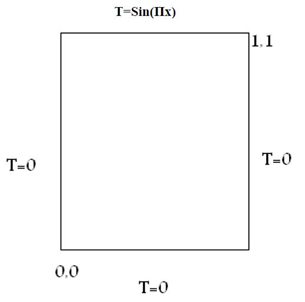
\includegraphics[width=0.4\textwidth]{figures/domain.png}
    \caption{Computational domain and prescribed boundary conditions.}
    \label{fig:domain}
\end{figure}

For the selected boundary conditions, an analytical solution exists and can therefore be used to verify the numerical implementation. The exact solution of Equation~\ref{eq:laplace} is

\begin{equation}
T(x,y)
=
\frac{\sin(\pi x)\sinh(\pi y)}
{\sinh(\pi)}
\label{eq:exact}
\end{equation}

The existence of the analytical solution given by Equation~\ref{eq:exact} makes this problem an ideal verification benchmark. Throughout this project, the numerical solution obtained using the finite-volume discretization and the Point Gauss-Seidel iterative solver is compared directly with the analytical temperature distribution to assess the correctness and accuracy of the numerical implementation.

